\section{Motivation}

\subsection{Resource Constraints}

\subsubsection{Characteristics of Wearable Cognitive Assistance Workload}
Wearable cognitive assistance applications are both latency-sensitive and
compute intensive. Latency-sensitivity is inherent to applications. The arrival
rate of instructions needs to match the time for humans to execute these
instructions. For instance, humans can recognize a person's face using around
1000~ms~\cite{kampf2002serial}. For a digital assistant that reminds a person
who a person is, the speed needs to be much faster than this value.

The high compute demand of wearable cognitive assistance comes from the
processing needs of modern computer vision algorithms. The accuracy of many
important computer vision tasks, such as object detection, image segmentation,
and face recognition, have been greatly improved since the advent of deep neural
networks (DNNs). While accuracy has improved, the computation demand has also
increased. Deep neural networks have tens to hundreds of perceptron layers and
millions of parameters. Both DNN train and inferencing involves millions of
multiply-and-add operations, which are implemented as matrix multiplication.
These large matrix multiplications have a high computational demand.

Previous measurements on wearable cognitive assistants provide quantitative
insights into both latency sensitivity and computation intensity.
Figure~\ref{table:application-bounds} shows latency requirements for seven
different applications. These applications serve a variety of purposes, from
guiding a user how to aim in a game of pool to teaching a user how to make a
sandwich. Chen et al.~\cite{chen2017empirical} describe how these bounds are
obtained. These latency requirements highlight the latency-sensitivity of
wearable cognitive assistants.

\begin{figure*}
\centering
\begin{tabular}{|l|c|c|c|c|c|c|c|}
\hline
                      & Pool & Work-out & Ping-pong & Face & Lego & Draw & Sandwich\\
\hline
    Tight Bound (ms) & 95 & 300 & 150 & 370 & \multicolumn{3}{c|}{600} \\
\hline
\end{tabular}
    \vspace{-0.0in}
    \caption{Application Latency Requirements}
\label{table:application-bounds}
\end{figure*}

\begin{figure*}
        \centering
    \begin{minipage}{5.3in}
        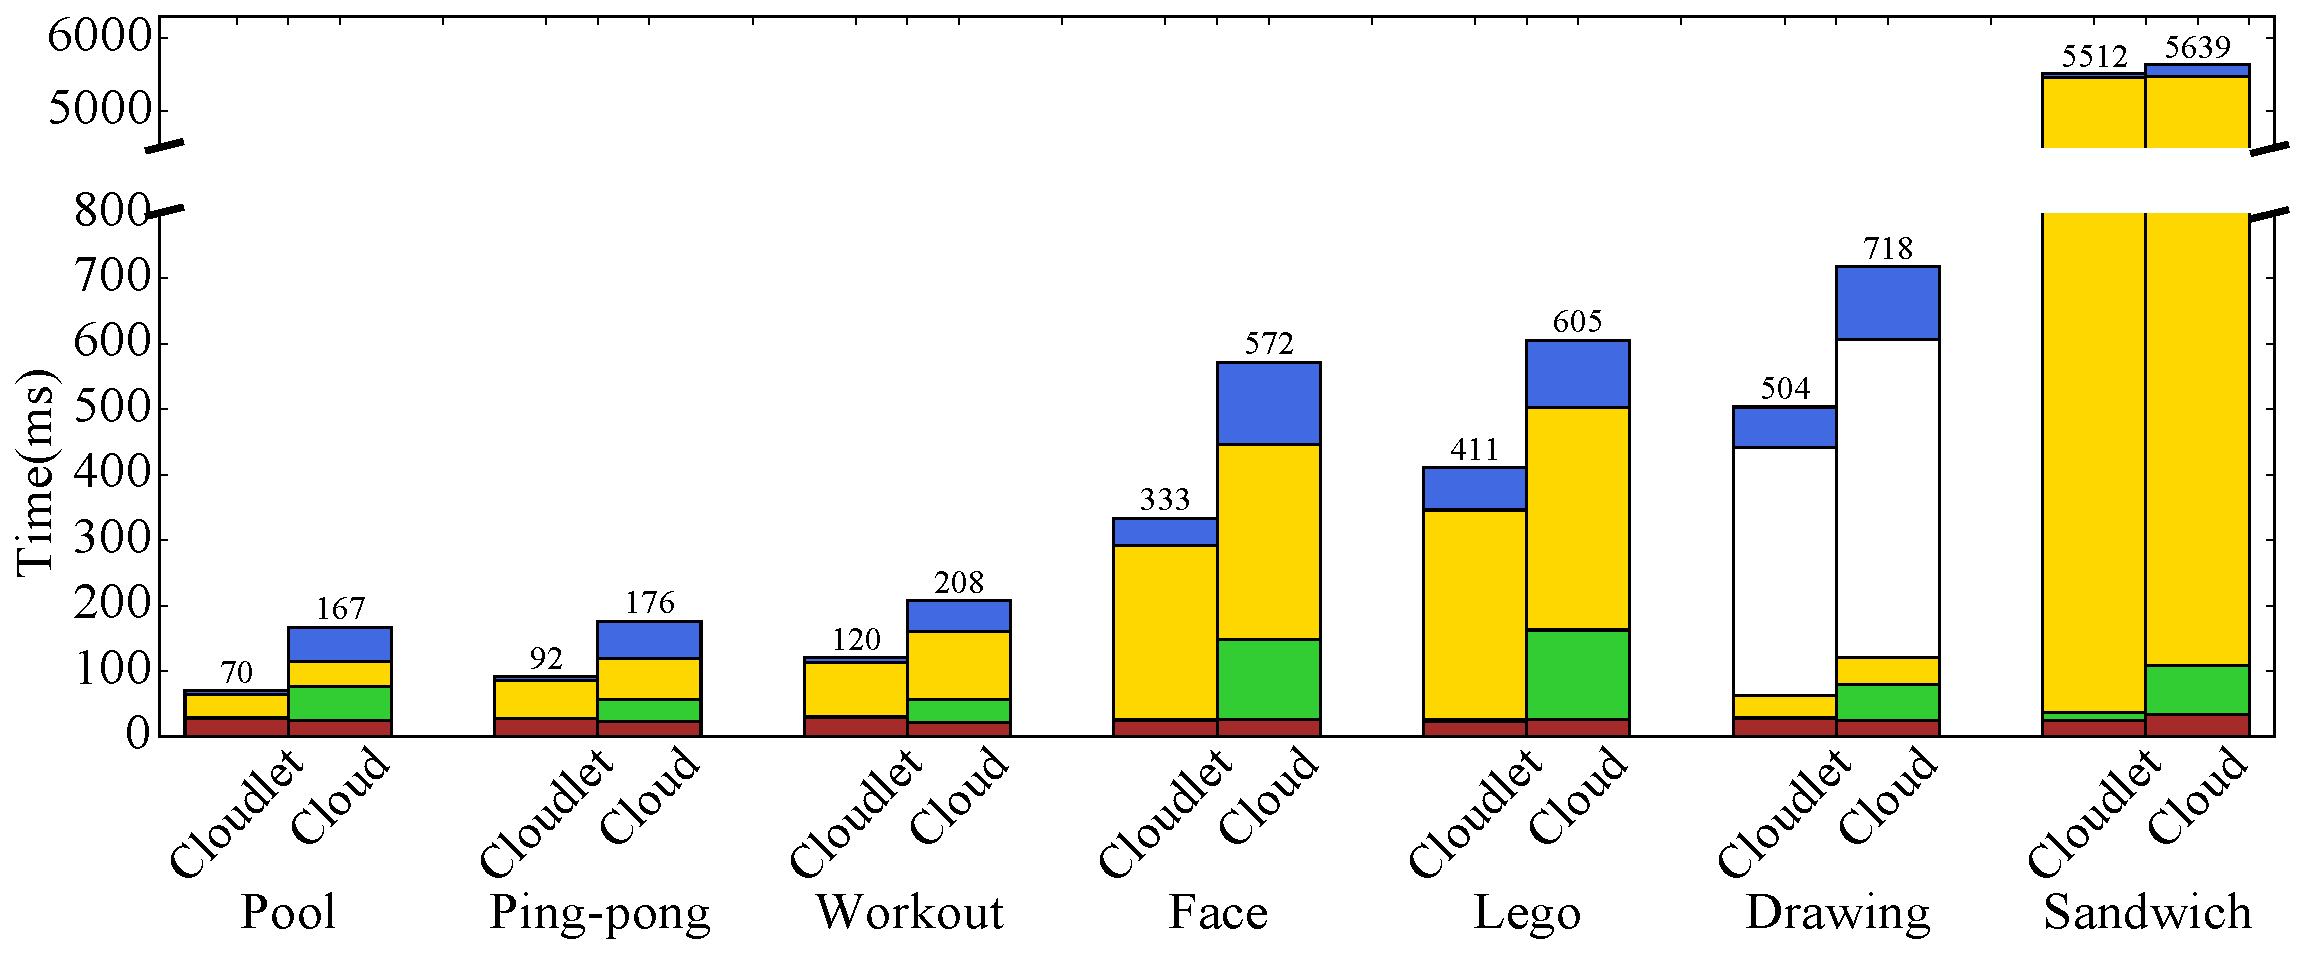
\includegraphics[height = 2in]{FIGS/pool-pingpong-workout-face-lego-draw-cooking-breakdown.pdf}
    \end{minipage}
    \hspace{-0.50in}
    \begin{minipage}{0.7in}
    \raisebox{0.5in}{
        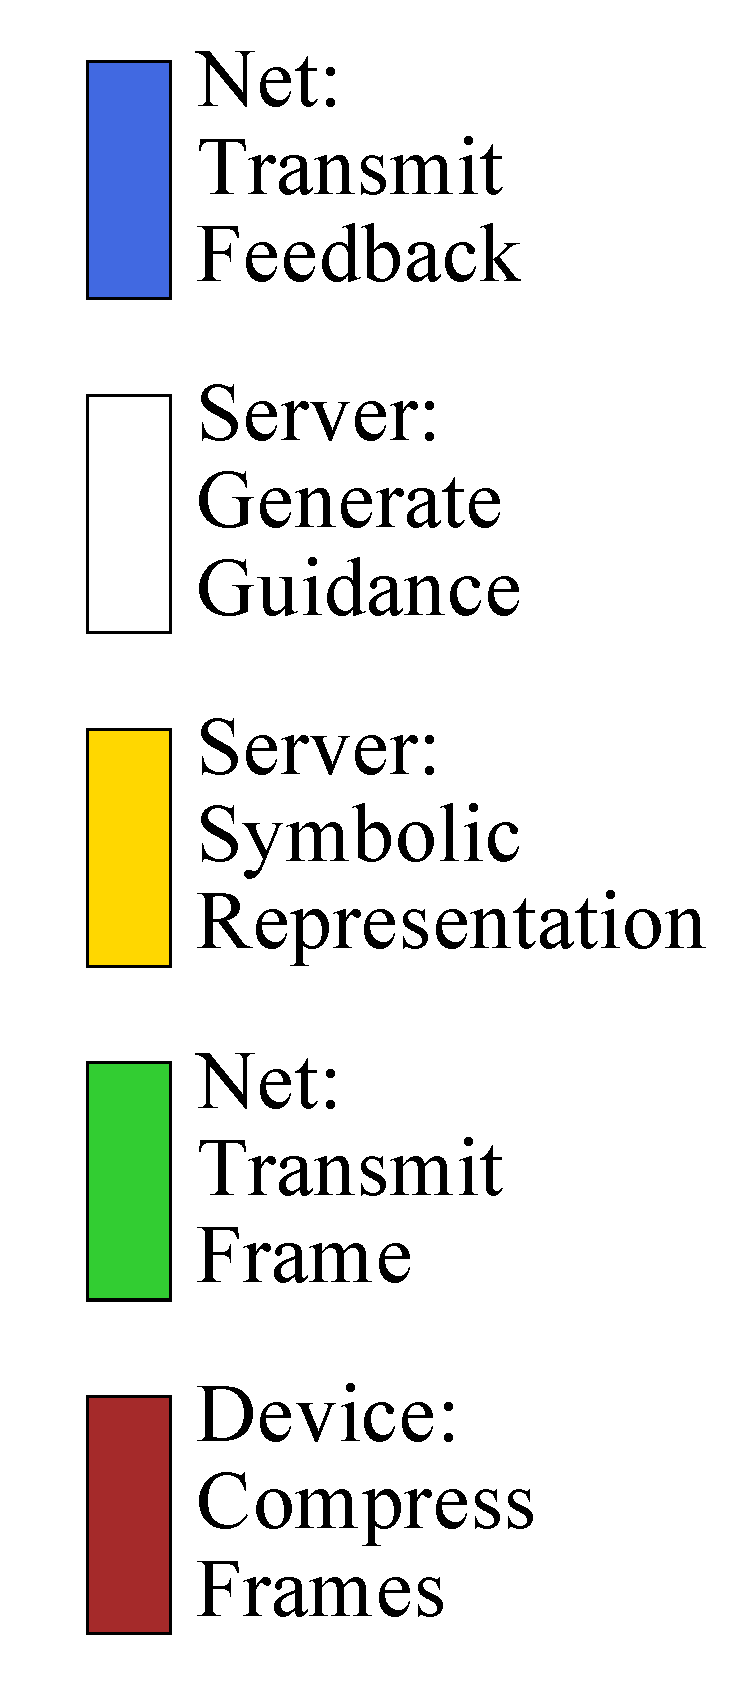
\includegraphics[height=1.9in]{FIGS/legend-breakdown.pdf}
    }
    \end{minipage}
    \vspace{-0.1in}
	\caption{Mean Latency Breakdown - Cloudlet vs. Cloud for Phone over WiFi}
    \vspace{-0.0in}
    \label{fig:breakdown}
\end{figure*}


Figure~\ref{fig:breakdown} shows the time breakdown of these assistants. For the
cloudlet case (left bars for each application), relatively little time is spent
on network transmission, which is the benefit of edge computing. When offloading
to the cloudlet, the server compute time consists of a significant portion, if
not the most significant part of the end-to-end latency. For applications
that use DNNs to process complex scenes, for example, Face and Sandwich, the
server computation time dominates.

\subsubsection{Wireless Network Characteristics}
The sensed data, e.g. images and videos from mobile devices, are transmitted to
a cloudlet through wireless communication. While IEEE 802.11 protocol is
widely-used at home and enterprise settings, the cellular network, particularly
LTE provides a better experience with its always-on ubiquitousness and large
area coverage. To this end, I will focus on LTE network as the primary wireless
communication protocol in the rest of my work.

LTE has unique characteristics in both latency and bandwidth. While previous
works~\cite{hu2016quantifying} and ~\cite{hadvzic2017edge} have experimentally
measured LTE's latency for mobile applications, the influence of LTE's bandwidth
and capacity on wearable cognitive assistance applications is mostly
unexplored.

The LTE uplink bandwidth is both limited and highly variant. LTE release 8 has a
theoretical a peak uplink data rate of 75 Mbps compared to 300 Mbps peak
downlink data rate. For LTE-Advanced, a major step toward 5G, the peak uplink
and downlink data rate are 1500 Mbps and 3000 Mbps respectively. In addition,
these theoretical peak data rates can only be achieved under idealized set-up
condition. For example, the LTE cell in test needs to be well isolated from
other cells while the test mobile device needs to be close to the base station.
Actual deployment has less bandwidth available~\cite{cox2012introduction}. For a
single user, the available bandwidth can be even less due to sharing. For
example, a 2012 study measured median LTE downlink and uplink bandwidth in US
commercial network to be 13 Mbps and 6 Mbps respectively~\cite{huang2012close}.
In 2017, the highest average upload bandwidth is 18 Mbps among providers in
US~\cite{PCMag2017}. In addition, LTE bandwidth has high
variance~\cite{winstein2013stochastic}. ~\cite{huang2012close} observed high
variation on LTE throughput not only for different users at different locations,
but also for the same user at the same location across different runs.

Gabriel applications put a high bandwidth demand on the network since they
continuously stream video data to cloudlets over wireless links. As a
comparison, Netflix recommends an internet connection speed of 5 Mbps to watch
its highly compressed HD video content. Gabriel applications would consume more
bandwidth due to on-the-fly compression. Hundreds of users simultaneously
streaming high-definition videos could easily saturate today's LTE uplink
capabilities~\cite{oyman2010toward}. Therefore, effective reduction of the
bandwidth consumption is essential to support concurrent running of many Gabriel
applications.

\subsection{Accelerators on Edge Nodes}
The computation capability of cloudlets, especially hardware accelerators, also
becomes a bottleneck with many users. The high demand for accelerator resources
comes from the widespread use of DNNs to solve computer vision tasks. DNNs'
superior learning ability enables them to advance the state-of-art accuracy. The
large capacity to learn comes from the sheer number of model parameters. For
example, the widely-used image classification network
ResNet-101~\cite{he2016deep} has more than 42 million parameters. Another
classifier network Inception ResNet V2 which achieves higher accuracy on
ImageNet~\cite{deng2009imagenet} has more than 53 million
parameters~\cite{huang2017speed}. For more sophisticated tasks, for example
object detection, additional layers are needed beyond image classifiers,
resulting in even more parameters. In addition, these networks are deep, with
tens to hundreds of layers in a sequence. Computational dependencies exist
among the bottom and top layers. The combined effect of a large number of both
parameters and layers is the high computational demands when using DNNs for
inference. In order to shorten computational latency, hardware accelerators that
can exploit parallel execution, for example GPUs, are commonly used for both
DNN training and inference. ASIC accelerators to further improve speed have also
been developed. For example, Google has deployed Tensor Processing Units (TPUs)
into their cloud to meet DNNs' computational
demands~\cite{jouppi2017datacenter}.

Despite many efforts in hardware design, the cost of DNN accelerators remains
high. For example, a Nvidia Pascal Titan X graphic card, a top-of-line GPU for
DNNs, costs around~\$1200~\cite{Nvidia2017TitanX}. Nevertheless, it can only run
the object detection network Faster-RCNN with ResNet101 at a speed of fewer than
10 frames per second (FPS)~\cite{huang2017speed}. Although large batch sizes
could theoretically improve the throughput, they often sacrifice application
latency and therefore are not suitable for many Gabriel applications. To support
more users with high demands on accelerators, Gabriel framework needs to
efficiently manage and share scarce and expensive acceleration resources among
concurrent users to reduce the cost of deployment.

\subsection{Difficulty of Development}

Gabriel applications are difficult to develop. Not only is the development
process slow, but specialized computer vision experience is also needed. It took
a researcher four months to build his first cognitive assistant for assembling
LEGO pieces~\cite{chen2018application}. The majority of time is spent on
learning the computer vision techniques and selecting robust algorithms to use
through trial and error. New developers would face the similar obstacles when
building these applications from scratch. As a result, the number of wearable
cognitive assistants available is quite limited. Therefore, Gabriel needs to be
extended with a toolchain to reduce the difficulty of development.

\begin{figure*}
  \centering
  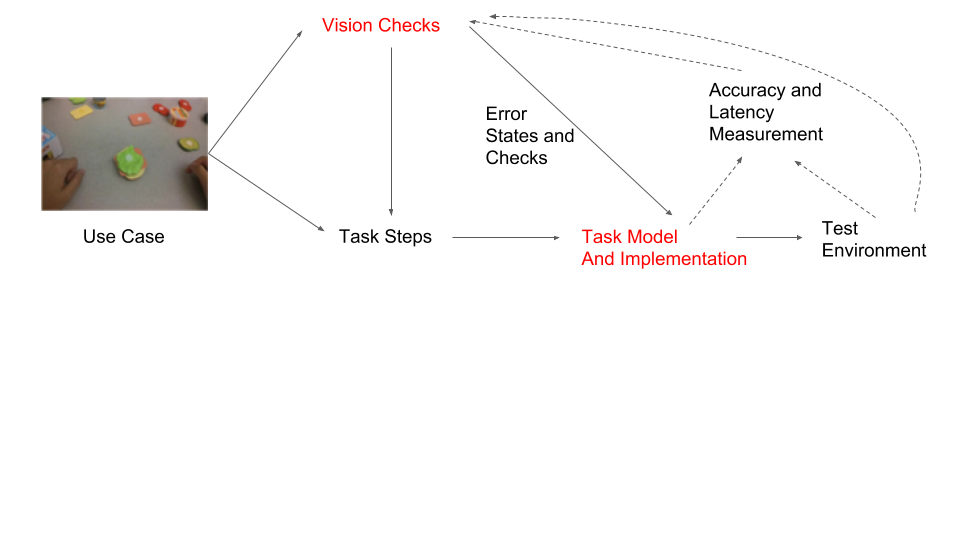
\includegraphics[trim={0 10cm 0 0},width=\linewidth]{FIGS/ad-hoc-workflow}
  \hspace{-0.50in}
	\caption{Development Workflow}
    \vspace{-0.0in}
    \label{fig:workflow}
\end{figure*}

The overall development workflow of wearable cognitive assistance is shown in
figure~\ref{fig:workflow}. After a use case is identified, developers would need
to identify meaningful visual states that can be detected using computer vision.
In the meantime, a task is divided into steps based on the use case and
detectable visual states. Task procedures could be changed to reduce the
difficulties of CV checks. In fact, since there is a human in the loop, relying
on humans to do what they are good at is the main reason that wearable cognitive
assistance can be implemented without solving perception and planning problems
intrinsic to robotics. Task procedures together with error states form a task
model. Developers implement the application according to the task model. After
 initial implementation, test runs and measurements are conducted to evaluate
the robustness of computer vision checks and end-to-end application latency.
This process is iterated until developers are satisfied.

Among all the development procedures, creating the computer vision checks to
detect user states consumes the most of development time and requires computer
vision expertise and experience. With the adoption of DNNs, developers no longer
need to spend days to select and tweak handcrafted features. Instead, the entire
model is trained end-to-end using labeled data. However, DNNs, with millions of
parameters to train, requires a significant amount of training data. Collecting
and labeling data are time-consuming and painstaking. Besides, to craft and
implement a DNN by hand is not trivial. Significant machine learning background
is needed to tweak network architectures and parameters. Therefore, developer
tools are needed to both help label the data and create deep neural networks.

In summary, implementing the workflow of cognitive assistance takes time and
efforts. Ad-hoc implementation requires a team of domain experts, developers and
computer vision experts. Such development model cannot scale to thousands of
applications. Therefore, Gabriel needs to be extended with tools to reduce the
effort of creating wearable cognitive assistants.
